\section{Implementation} \label{sec:Implementation}

The initial Minimum Viable Product (MVP) was implemented with major
differences from the design outlined in chapter \ref{sec:AnalysisAndDesign}.
The most visible one is the fact that (what is mainly) the \emph{Mediator}
pattern (\cite[][Ch.~9,~Location~3594]{nikolov2016scala}) has been used in
order to implement the dialogue between the presentation and other layers using
a feature which resembles the MVC architecture. Normally, this type of
architecture is implemented in order to make sure that multiple views can refer
to the same core functionality (or model) without actually implementing that
functionality themselves, which allows the view to be responsible for
presentation and the model for liaising with the business logic through a
controller. This also allows the controller to update multiple existing views
based on what input was received from one view
(\cite[][p.~381]{bennett2010object}). The difference in the implementation for
this project is that this last feature, essentially, was not implemented, since
only one view exists at one time.

In the implementation phase of this project, the components were segregated
into packages (each of which represents one of the layers mentioned in Chapter
\ref{sec:AnalysisAndDesign}) and sub-packages. Each sub-package has been
implemented so that it does not have any knowledge of the super-package, but
rather exposes and depends on interfaces which exist within itself. The
super-packages, then, implement the interfaces of the sub-packages, which
allows them to interact with the sub-package components. The \emph{Mediator}
pattern was implemented at the default package level by the
\emph{InteractionMediator} and \emph{PersistenceMediator} objects, both of
which also happen to represent Scala's native implementation of the
\emph{Singleton} pattern (\cite[][Ch.~6,~Location.~2242]{nikolov2016scala}).
The following subsections will give more detail into the inner workings of the
application and the techniques used to build it.

\subsection{Presentation Layer} \label{sec:Implementation.Presentation}
In the presentation layer, for this MVP, the \emph{Scala Swing} package was
used to design the \emph{view}. The package itself consists of Scala wrappers
for the \emph{Java Swing} package, and one of the reasons why it was chosen was
that, as with many other GUI packages, it already comes with an implementation
of the \emph{Observer Design Pattern} (\cite[][p.~293]{gamma1995design}) in its
capacity to react to events (\cite[][p.~5]{maier2009scala};
\cite[][Ch.~9,~Location~3731]{nikolov2016scala}).

The entry point of the application is the \texttt{App} object, in the main
package. This application works as a main method, and its only task is to
call the \texttt{InteractionMediator.startup} method, which will send a
message through the \texttt{PresentationMediator} instance returned by the
\texttt{PresentationBuilder} to start the view.

\begin{sloppypar}
  In its current implementation, the view is started by the \texttt{MainWindow}
  class, which extends the \texttt{scala.swing.MainFrame} class. A
  \texttt{MainFrame} is a Swing \texttt{Frame} -- ``a window containing
  arbitrary data'' (\cite[][Ch.~34,~Section~34.1]{odersky2016scala}) -- that
  can send a signal to terminate the application when closed.
  \texttt{MainWindow} also has implementations of other methods to allow the
  application to close gracefully, all of which were inspired by the
  \texttt{SimpleSwingApplication} of the scala package
  (\cite[][p.~2~\&~3]{maier2009scala}). The author chose not to make the first
  extend the latter was because the super-class implements a main method,
  which, considering that it would be another entry point to the application,
  could cause confusion when it were to start (not to mention the fact that
  this is not the responsibility of the \texttt{MainWindow} class).
\end{sloppypar}


As mentioned in the beginning of this chapter, each sub-package has been
designed so that it does not have to depend on the packages which envelop it.
The diagram below (Figure \ref{fig:PresentationMVC}) illustrates this using the
interaction between the \texttt{InteractionMediator}, \texttt{SwingAmbassador}
and the \texttt{presentation.swing} package and sub-packages as an example:

\begin{figure}[ht!]
  \begin{center}
    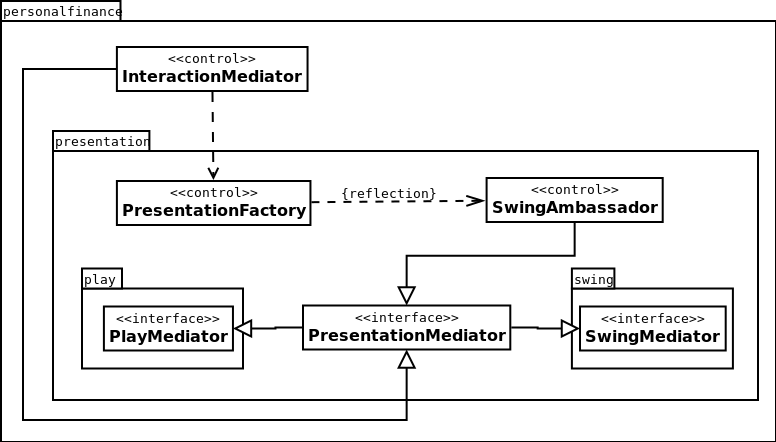
\includegraphics[width=15cm]{contents/img/Package_Diagram_-_Presentation_MVC.png}
  \end{center}
  \caption{}
  \label{fig:PresentationMVC}
\end{figure}
\FloatBarrier


\begin{sloppypar}
  In order to preserve encapsulation, specifically for the \texttt{swing}
  package, only the \texttt{MainWindow} controller and \texttt{SwingMediator}
  interface are exposed to the outside world, with the first having a
  constructor dependency on the latter. This means that, in order to interact
  with the components of the package, any external classes will need to
  implement the \texttt{SwingMediator} interface. This is also useful if the
  \texttt{presentation.swing} package is to be extracted and used as a library
  in another project, and also leaves room for the \emph{Adaptor} pattern
  (\cite[][p.~139]{gamma1995design}), if it needs to interact with other
  objects which do not necessarily implement the interface upon which it
  depends.
\end{sloppypar}

One feature also noticeable in Figure \ref{fig:PresentationMVC} is the fact the
\texttt{personalfinance} package is unaware of which of the view's
implementation it is interacting with. The modified version of 
\emph{Builder} pattern (\cite[][pp.~37-38]{lokke2009scala}) implemented on
\texttt{PresentationBuilder}, which uses reflection to determine what
implementation to build, allows for the view itself to be decided with the use
of an external \texttt{.properties} file. This allows for the actual
implementation which will be delivered by the Factory to change without the
code having to be recompiled, which introduces flexibility to the application.
The \texttt{play} package is only a placeholder at this point, as due to time
constraints it was not possible to actually implement it, but it is there to
exemplify how the project can be further extended.

Another element not seen in the diagram but which is present in the code is the
fact that the dependency of the \texttt{MainWindow} class on the
\texttt{SwingMediator} interface exists in the constructor, as seen in the code
listing below:
{
  \small
  \lstinputlisting[
    language=Scala,
    firstline=7,
    lastline=7,
    caption={ }
  ]{../code/src/main/scala/personalfinance/presentation/swing/MainWindow.scala}
}

This is an attempt at implementing the principle of \emph{Dependency Injection}
through \emph{Constructor Injection} (\cite[][]{fowler2004inversion}). In the
case of this project, the advantage of this simple piece of code is tremendous,
especially because the fact that the \texttt{MainWindow} class does not have to
instantiate a mediator -- it simply relies on the fields published by the
\texttt{SwingMediator} trait. Likewise, the fact that the
\texttt{InteractionMediator} singleton object has a dependency on the
\texttt{PresentationBuilder} only, allows for the actual implementation of the
view to change without it having to change.


\textbf{Talk how the above is a risky move, since Scala's mixin composition has
this habit of picking up the implementation of the last trait mixed into it, so
in this case you get PresentationMediator inheriting form SwingMediator and
then PlayMediator -- although both are traits, this could cause problems in the
future if the Play one implements something which Swing doesn't, so basically
these traits must always be the exact same}

\textbf{talk about the reason why the presentation mediator's methods returning
Unit being because this way they can stay as implementation-agnostic regarding
the other layers as they possibly can, again thinking that the interface needs
to be able to change without the code being recompiled}



\subsection{Business Logic} \label{sec:Implementation.BusinessLogic}

The business logic layer is the one which adhered more firmly to the model
designed in section
\ref{sec:AnalysisAndDesign.BusinessLogic.FinalClassDiagram}. The following are
a few highlights from the implementation which are worth mentioning.

\subsubsection{Scala Case Classes and the Prototype Design Pattern} \label{sec:Implementation.ScalaCaseClasses}
One of the benefits of Scala are its case classes. Not just are they very
useful for pattern matching, but also come with a few perks such as the
\texttt{copy} method. This method allows for an object to be copied with some
or all its members modified. It could be said that it is a language-native
implementation of the \emph{Prototype Design Pattern}
(\cite[][Ch.~6,~Location~2461]{nikolov2016scala}), and throughout the
implementation and testing stage it proved to be a useful asset.

One of its many utilisations can be seen in the \texttt{Transaction} class, as
one of the tools used to add entries to a \texttt{Category} without having to
change the state of a specific instance -- more similar to what is done in the
\emph{Functional Programming} paradigm:
{
  \small
  \lstinputlisting[
    language=Scala,
    firstline=35,
    lastline=40,
    caption={
      extract of the \texttt{Transaction} class showing the \texttt{copy()}
      method in action
    }
  ]{../code/src/main/scala/personalfinance/businesslogic/transaction/Transaction.scala}
}


\textbf{TODO: write about why Validator has an auxiliary method for type --
generics would affect the interface. The Validator was created as a trait in
the first place to allow for lesser coupling between the classes which need
validation}


In order to be concise where possible, where it was felt that the domain's
requirements were captured accurately and was estimated that they are not
likely to change, high level modules are depending directly on classes rather
than interfaces. This can be seen as being in direct violation of the
\emph{Dependency Inversion} principle of SOLID
(\cite[][]{martin1996dependency}), which some would consider to be a ``risky'''
move (after all, it is not always possible to predict which requirements will
and which will not change), but others would believe that this was acceptable
for more static requirements. The author decided to follow the latter.

\begin{sloppypar}
  However, this principle was still employed where it seemed beneficial to
  follow it -- for example, in areas where it was felt that the implementation
  of certain algorithms could be further optimised in future iterations. This
  is the case with \texttt{transaction.RegexDateStringParser}: this class
  implements the \texttt{transaction.dates.DateStringParser} trait, upon which
  the higher level modules which use dates will depend. This is an example of
  one of the places in the code where the \emph{Dependency Inversion} principle
  can be seen, but it is not the only one.
\end{sloppypar}


\subsubsection{The engine behind it all: the \texttt{Classifier}}

Another example of \emph{Dependency Inversion} (though not of \emph{Dependency
Injection}) is the \texttt{Classifier} trait, and the class implementing it:
\texttt{StringClassifier}. The \texttt{InteractionMediator} declares a variable
of the first type, and then instantiates it with the latter. Therefore,
although it still depends on the abstraction, it also has a dependency on the
implementation, which would mean that in order to change it a slight
refactoring would be necessary.

For this implementation, \texttt{StringClassifier} was built using longest matching
prefix to match entries to categories: patterns are matched to the start of the
description of every entry, starting from longest pattern to the shortest. This
is so that if there is, for example, a pattern ``Laptop for parent'' which
would match to category ``Gifts'', and another pattern ``laptop'', for category
``personal equipment'', then entries with the description ``Laptop for
Girlfriend'' would not be picked up by the shorter match for laptop. Below is a
code listing which shows how this was implemented:
{
  \small
  \lstinputlisting[
    language=Scala,
    firstline=30,
    lastline=60,
    caption={
      Extract of the \texttt{StringClassifier} class, showing the algorithm currently
      used to match Entry descriptions' prefixes against patterns
    }
  ]{../code/src/main/scala/personalfinance/businesslogic/Classifier.scala}
}

As mentioned on the code listing above, the \emph{longest matching prefix} is
achieved by sorting all the patterns by length, from longest to shortest, then
trying to match them against the prefix of the entry description in the same
order. This way, even if an entry would be a match against more than one
category, the pattern with the longest matching prefix will still be the first
match.

One other interesting feature which can be seen in the above listing is how
much is being done using the native \texttt{flatMap} and \texttt{foldLeft}
methods of Scala collections. The \texttt{map} function and its derivates are
normally implemented by types which can be classified as \emph{Functors} in
scala. Functors are challenging to explain concisely, but for this report it
should suffice to say that they are \emph{classes which implement the}
\texttt{map} \emph{method and conform to a set of laws called} \textbf{functor
laws}. The \texttt{foldLeft} method of the collections are also an indication
that they can be classified as \emph{monoids}, which are another construct
brought over from mathematics. The main point of mentioning these is because
they are one of the things which makes the functional paradigm so powerful:
these constructs create a common interface which allows for the different types
with which they are associated to be interacted with in a common way -- that
is, a lot can be done with them with very few lines of code
(\cite[][Ch.~1,~Location~4243~\&~703]{nikolov2016scala}). Not just this, but
the immutability of the instances within them also makes it easy to perform
these operations in parallel and, although this parallelism has not been
explicitly implemented in this iteration, the author felt it was worth
mentioning them in this section.

\subsection{The Presentation Layer}

The presentation layer is another one where decoupling and reflection can be
observed. The package is accessible via the \texttt{PersistenceBridge} class,
which uses reflection to instantiate one of the classes which implements the
\texttt{ConnectionType} trait. This is an implementation of the \emph{Strategy}
pattern (\cite[][p.~80]{lokke2009scala}), which allows for the database vendor
to be changed without the code having to be recompiled. At the moment, the only
dialect implemented is \emph{MySQL}, but a placeholder can already be seen for
the \emph{H2} database.

It is also worth noticing that the operations currently being executed by the
implementation have a lot of room for improvement: many of the queries and
updates which could be grouped together and sent to the database in batch are
still being done individually. This does not have a huge impact on performance
with a local database, but might cause issues with remote ones. Further
iterations of the application should focus on optimising this.

Another pattern which can be observed in this layer is the \emph{Value Object}
pattern, which will be discussed in more detail below.

\subsubsection{Algebraic Data Types and the Value Object Pattern} \label{sec:Implementation.ADTAndValueObject}
Throughout the code, examples of Algebraic Data Types can be seen. These appear
in the form of sealed traits and case objects, and are normally used when
instances need to be passed around as values, but also contain information which will
be relevant to the code. Examples of these can be found in the
\texttt{ConnectionType} hierarchy, where the number of possible instances for
each case class would classify the trait and its subtypes as \emph{Product
Types} (\cite[][p.~411]{wampler2015programming}). The code listing below
illustrates this:

{
  \small
  \lstinputlisting[
    language=Scala,
    firstline=9,
    lastline=9,
    caption={
      extract of the \texttt{ConnectionType} hierarchy showing the case classes
      used as value objects
    }
  ]{../code/src/main/scala/personalfinance/persistence/connections/ConnectionType.scala}
}
...

{
  \small
  \lstinputlisting[
    language=Scala,
    firstline=39,
    lastline=40
  ]{../code/src/main/scala/personalfinance/persistence/connections/ConnectionType.scala}
}
...

{
  \small
  \lstinputlisting[
    language=Scala,
    firstline=90,
    lastline=91
  ]{../code/src/main/scala/personalfinance/persistence/connections/ConnectionType.scala}
}
...

Algebraic data types could be said to be the natural implementation of the
Value Object design pattern. This pattern is used widely for comparison of
objects not by their identities, but rather by their values. They consist of
small, immutable objects, and the instances of the case classes can be
classified as just those (\cite[][Ch.~8,~Location~3068]{nikolov2016scala}).
